\section{Exercise 1: Perceptron}
\subsection{Part a}
To have an idea of what our perceptron looks like, let's plot its discriminant line
and the two data points.
\\
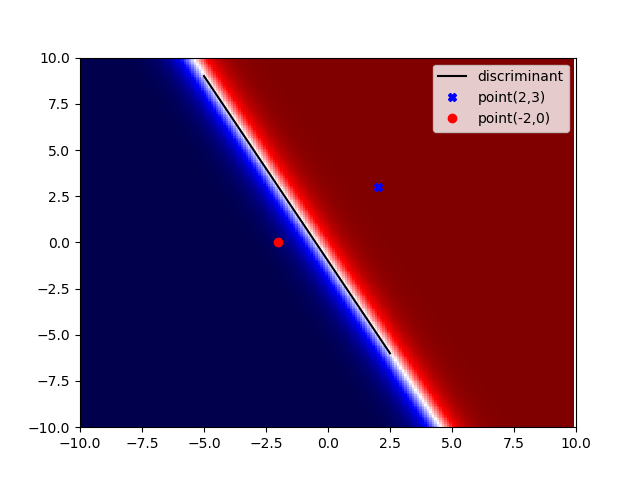
\includegraphics[scale=0.6]{ex1_a.png}
\\
We can also compute the prediction of the model for the two datapoints:
$$
\text{prediction}_1 = sign(w^\top x_1) = sign(8) = 1 \ne -1
$$
$$
\text{prediction}_2 = sign(w^\top x_2) = sign(-3) = -1 \ne 1
$$
So our two datapoints are missclassified, now we can say that on the plot below 
area in red (upper right of the plot) represents the area classified as class $1$ by our model and
blue (lower left part of the plot) is for class $-1$

\subsection{Part b}
After one iteration of a batch learning algorithm we get the following new discriminant:
$$
w_{new} = w_{old} + \eta\sum_{i=1}^N x_ic_i
$$
$$
w_{new} = \begin{bmatrix}1 & 0 & -0.5\end{bmatrix}
$$
And now, both data points are acorrectly classified by the new model:
\\
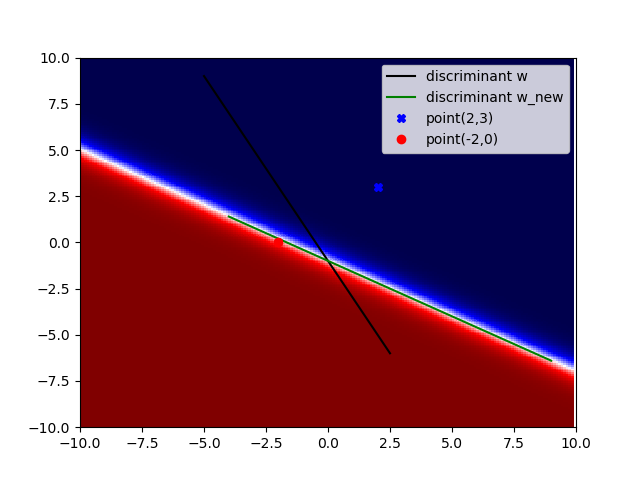
\includegraphics[scale=0.6]{ex1_b.png}

\subsection{Part c}
Learning is an iterative process. In a batch version learning, at each iteration we compute a new model
based on the whole dataset whereas in a stochastic version, at each iteration we pick up a single data in the dataset
and we base our computation on this data point only.
\\
When the dataset becomes too big, the computation time of a batch iteration is going to need ressources 
proportional to the size of the dataset and a stochastic iteration will always use the same amount of ressources
independantly of the size of the dataset.

\subsection{Part d}
When applying the stochastic algorithm, we get the following (different) result:
$$
w_{new} = \begin{bmatrix}1 & -0.4 & -0.8\end{bmatrix}
$$
And again, both points are correctly classified after the complete sweep:
\\
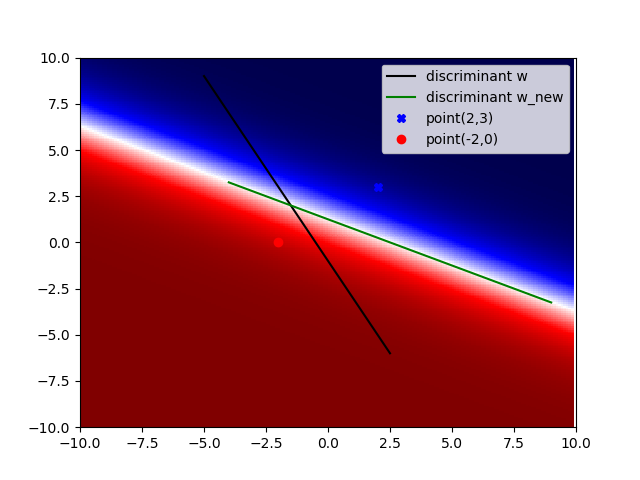
\includegraphics[scale=0.6]{ex1_d.png}


\section{Exercise 3: Error function \& Gradient descent}
\subsection{Part a}
If $y_n = \sigma(w^\top x_n)$ then:
$$
E(w) = \sum_{n=1}^N (t_n-y_n)^4
$$
$$
\nabla_w E(w) = -4\sum_{n=1}^N (t_n-y_n)^3(y_n (1-y_n))x_n
$$

\subsection{Part b}
$$
E(w) = \sum_{n=1}^N \vert t_n - y_n \vert
$$
Computing the gradient of an absolute value implies to derivate an
absolute value function which  is not $C^1$. We won't be able to assign 
a value to the gradient if the value inside the absolute function is 0.
$$
\nabla_w E(w) = \sum_{n=1}^N \left\{ \begin{array}{ll}  
                    -y_n(1-y_n)x_n & \text{if $t_n-y_n > 0$}
                \\ 
                    y_n(1-y_n)x_n & \text{if $t_n-y_n < 0$}
                        \end{array}
                \right.
$$